%%%%%%%%%%%%%%%%%%%%%%%%%%%%%%%%%%%%%%%%%
% The Legrand Orange Book
% LaTeX Template
% Version 2.3 (8/8/17)
%
%
% License:
% CC BY-NC-SA 3.0 (http://creativecommons.org/licenses/by-nc-sa/3.0/)
%
% Compiling this template:
% This template uses biber for its bibliography and makeindex for its index.
% When you first open the template, compile it from the command line with the 
% commands below to make sure your LaTeX distribution is configured correctly:
%
% 1) pdflatex main
% 2) makeindex main.idx -s StyleInd.ist
% 3) biber main
% 4) pdflatex main x 2
%
% After this, when you wish to update the bibliography/index use the appropriate
% command above and make sure to compile with pdflatex severa
% This template has been downloaded from:
% http://www.LaTeXTemplates.com
% This template also uses a number of packages which may need to be
% updated to the newest versions for the template to compile. It is strongly
% recommended you update your LaTeX distribution if you have any
% compilation errors.
%
% Important note:
% Chapter heading images should have a 2:1 width:height ratio,
% e.g. 920px width and 460px height.
%
%%%%%%%%%%%%%%%%%%%%%%%%%%%%%%%%%%%%%%%%%

%----------------------------------------------------------------------------------------
%	PACKAGES AND OTHER DOCUMENT CONFIGURATIONS
%----------------------------------------------------------------------------------------

\documentclass[11pt,fleqn]{book} % Default font size and left-justified equations

%----------------------------------------------------------------------------------------
\usepackage{listings}
\usepackage{xcolor}
\usepackage{caption}
\usepackage{makecell}
\usepackage{tikz}
\usepackage{float}
\usetikzlibrary{arrows, chains}
\lstset {
	language=C++,
	backgroundcolor=\color{black!5},
	basicstyle=\footnotesize,
	frame=tb,
	tabsize=4,
	showstringspaces=false,
	commentstyle=\color{green},
	keywordstyle=\color{blue},
	stringstyle=\color{red},
}
%%%%%%%%%%%%%%%%%%%%%%%%%%%%%%%%%%%%%%%%%
% The Legrand Orange Book
% Structural Definitions File
% Version 2.0 (9/2/15)
%
% Original author:
% Mathias Legrand (legrand.mathias@gmail.com) with modifications by:
% Vel (vel@latextemplates.com)
% 
% This file has been downloaded from:
% http://www.LaTeXTemplates.com
%
% License:
% CC BY-NC-SA 3.0 (http://creativecommons.org/licenses/by-nc-sa/3.0/)
%
%%%%%%%%%%%%%%%%%%%%%%%%%%%%%%%%%%%%%%%%%

%----------------------------------------------------------------------------------------
%	VARIOUS REQUIRED PACKAGES AND CONFIGURATIONS
%----------------------------------------------------------------------------------------

\usepackage[top=3cm,bottom=3cm,left=3cm,right=3cm,headsep=10pt,a4paper]{geometry} % Page margins

\usepackage{graphicx} % Required for including pictures
\graphicspath{{Pictures/}} % Specifies the directory where pictures are stored

\usepackage{lipsum} % Inserts dummy text

\usepackage{tikz} % Required for drawing custom shapes

\usepackage[english]{babel} % English language/hyphenation

\usepackage{enumitem} % Customize lists
\setlist{nolistsep} % Reduce spacing between bullet points and numbered lists

\usepackage{booktabs} % Required for nicer horizontal rules in tables

\usepackage{xcolor} % Required for specifying colors by name
\definecolor{ocre}{RGB}{225,100,225} % Define the orange color used for highlighting throughout the book

%----------------------------------------------------------------------------------------
%	FONTS
%----------------------------------------------------------------------------------------

\usepackage{avant} % Use the Avantgarde font for headings
%\usepackage{times} % Use the Times font for headings
\usepackage{mathptmx} % Use the Adobe Times Roman as the default text font together with math symbols from the Sym­bol, Chancery and Com­puter Modern fonts

\usepackage{microtype} % Slightly tweak font spacing for aesthetics
\usepackage[utf8]{inputenc} % Required for including letters with accents
\usepackage[T1]{fontenc} % Use 8-bit encoding that has 256 glyphs

%----------------------------------------------------------------------------------------
%	BIBLIOGRAPHY AND INDEX
%----------------------------------------------------------------------------------------

\usepackage[style=numeric,citestyle=numeric,sorting=nyt,sortcites=true,autopunct=true,babel=hyphen,hyperref=true,abbreviate=false,backref=true,backend=biber]{biblatex}
\addbibresource{bibliography.bib} % BibTeX bibliography file
\defbibheading{bibempty}{}

\usepackage{calc} % For simpler calculation - used for spacing the index letter headings correctly
\usepackage{makeidx} % Required to make an index
\makeindex % Tells LaTeX to create the files required for indexing

%----------------------------------------------------------------------------------------
%	MAIN TABLE OF CONTENTS
%----------------------------------------------------------------------------------------

\usepackage{titletoc} % Required for manipulating the table of contents

\contentsmargin{0cm} % Removes the default margin

% Part text styling
\titlecontents{part}[0cm]
{\addvspace{20pt}\centering\large\bfseries}
{}
{}
{}

% Chapter text styling
\titlecontents{chapter}[1.25cm] % Indentation
{\addvspace{12pt}\large\sffamily\bfseries} % Spacing and font options for chapters
{\color{ocre!60}\contentslabel[\Large\thecontentslabel]{1.25cm}\color{ocre}} % Chapter number
{\color{ocre}}  
{\color{ocre!60}\normalsize\;\titlerule*[.5pc]{.}\;\thecontentspage} % Page number

% Section text styling
\titlecontents{section}[1.25cm] % Indentation
{\addvspace{3pt}\sffamily\bfseries} % Spacing and font options for sections
{\contentslabel[\thecontentslabel]{1.25cm}} % Section number
{}
{\hfill\color{black}\thecontentspage} % Page number
[]

% Subsection text styling
\titlecontents{subsection}[1.25cm] % Indentation
{\addvspace{1pt}\sffamily\small} % Spacing and font options for subsections
{\contentslabel[\thecontentslabel]{1.25cm}} % Subsection number
{}
{\ \titlerule*[.5pc]{.}\;\thecontentspage} % Page number
[]

% List of figures
\titlecontents{figure}[0em]
{\addvspace{-5pt}\sffamily}
{\thecontentslabel\hspace*{1em}}
{}
{\ \titlerule*[.5pc]{.}\;\thecontentspage}
[]

% List of tables
\titlecontents{table}[0em]
{\addvspace{-5pt}\sffamily}
{\thecontentslabel\hspace*{1em}}
{}
{\ \titlerule*[.5pc]{.}\;\thecontentspage}
[]

%----------------------------------------------------------------------------------------
%	MINI TABLE OF CONTENTS IN PART HEADS
%----------------------------------------------------------------------------------------

% Chapter text styling
\titlecontents{lchapter}[0em] % Indenting
{\addvspace{15pt}\large\sffamily\bfseries} % Spacing and font options for chapters
{\color{ocre}\contentslabel[\Large\thecontentslabel]{1.25cm}\color{ocre}} % Chapter number
{}  
{\color{ocre}\normalsize\sffamily\bfseries\;\titlerule*[.5pc]{.}\;\thecontentspage} % Page number

% Section text styling
\titlecontents{lsection}[0em] % Indenting
{\sffamily\small} % Spacing and font options for sections
{\contentslabel[\thecontentslabel]{1.25cm}} % Section number
{}
{}

% Subsection text styling
\titlecontents{lsubsection}[.5em] % Indentation
{\normalfont\footnotesize\sffamily} % Font settings
{}
{}
{}

%----------------------------------------------------------------------------------------
%	PAGE HEADERS
%----------------------------------------------------------------------------------------

\usepackage{fancyhdr} % Required for header and footer configuration

\pagestyle{fancy}
\renewcommand{\chaptermark}[1]{\markboth{\sffamily\normalsize\bfseries\chaptername\ \thechapter.\ #1}{}} % Chapter text font settings
\renewcommand{\sectionmark}[1]{\markright{\sffamily\normalsize\thesection\hspace{5pt}#1}{}} % Section text font settings
\fancyhf{} \fancyhead[LE,RO]{\sffamily\normalsize\thepage} % Font setting for the page number in the header
\fancyhead[LO]{\rightmark} % Print the nearest section name on the left side of odd pages
\fancyhead[RE]{\leftmark} % Print the current chapter name on the right side of even pages
\renewcommand{\headrulewidth}{0.5pt} % Width of the rule under the header
\addtolength{\headheight}{2.5pt} % Increase the spacing around the header slightly
\renewcommand{\footrulewidth}{0pt} % Removes the rule in the footer
\fancypagestyle{plain}{\fancyhead{}\renewcommand{\headrulewidth}{0pt}} % Style for when a plain pagestyle is specified

% Removes the header from odd empty pages at the end of chapters
\makeatletter
\renewcommand{\cleardoublepage}{
\clearpage\ifodd\c@page\else
\hbox{}
\vspace*{\fill}
\thispagestyle{empty}
\newpage
\fi}

%----------------------------------------------------------------------------------------
%	THEOREM STYLES
%----------------------------------------------------------------------------------------

\usepackage{amsmath,amsfonts,amssymb,amsthm} % For math equations, theorems, symbols, etc

\newcommand{\intoo}[2]{\mathopen{]}#1\,;#2\mathclose{[}}
\newcommand{\ud}{\mathop{\mathrm{{}d}}\mathopen{}}
\newcommand{\intff}[2]{\mathopen{[}#1\,;#2\mathclose{]}}
\newtheorem{notation}{Notation}[chapter]

% Boxed/framed environments
\newtheoremstyle{ocrenumbox}% % Theorem style name
{0pt}% Space above
{0pt}% Space below
{\normalfont}% % Body font
{}% Indent amount
{\small\bf\sffamily\color{ocre}}% % Theorem head font
{\;}% Punctuation after theorem head
{0.25em}% Space after theorem head
{\small\sffamily\color{ocre}\thmname{#1}\nobreakspace\thmnumber{\@ifnotempty{#1}{}\@upn{#2}}% Theorem text (e.g. Theorem 2.1)
\thmnote{\nobreakspace\the\thm@notefont\sffamily\bfseries\color{black}---\nobreakspace#3.}} % Optional theorem note
\renewcommand{\qedsymbol}{$\blacksquare$}% Optional qed square

\newtheoremstyle{blacknumex}% Theorem style name
{5pt}% Space above
{5pt}% Space below
{\normalfont}% Body font
{} % Indent amount
{\small\bf\sffamily}% Theorem head font
{\;}% Punctuation after theorem head
{0.25em}% Space after theorem head
{\small\sffamily{\tiny\ensuremath{\blacksquare}}\nobreakspace\thmname{#1}\nobreakspace\thmnumber{\@ifnotempty{#1}{}\@upn{#2}}% Theorem text (e.g. Theorem 2.1)
\thmnote{\nobreakspace\the\thm@notefont\sffamily\bfseries---\nobreakspace#3.}}% Optional theorem note

\newtheoremstyle{blacknumbox} % Theorem style name
{0pt}% Space above
{0pt}% Space below
{\normalfont}% Body font
{}% Indent amount
{\small\bf\sffamily}% Theorem head font
{\;}% Punctuation after theorem head
{0.25em}% Space after theorem head
{\small\sffamily\thmname{#1}\nobreakspace\thmnumber{\@ifnotempty{#1}{}\@upn{#2}}% Theorem text (e.g. Theorem 2.1)
\thmnote{\nobreakspace\the\thm@notefont\sffamily\bfseries---\nobreakspace#3.}}% Optional theorem note

% Non-boxed/non-framed environments
\newtheoremstyle{ocrenum}% % Theorem style name
{5pt}% Space above
{5pt}% Space below
{\normalfont}% % Body font
{}% Indent amount
{\small\bf\sffamily\color{ocre}}% % Theorem head font
{\;}% Punctuation after theorem head
{0.25em}% Space after theorem head
{\small\sffamily\color{ocre}\thmname{#1}\nobreakspace\thmnumber{\@ifnotempty{#1}{}\@upn{#2}}% Theorem text (e.g. Theorem 2.1)
\thmnote{\nobreakspace\the\thm@notefont\sffamily\bfseries\color{black}---\nobreakspace#3.}} % Optional theorem note
\renewcommand{\qedsymbol}{$\blacksquare$}% Optional qed square
\makeatother

% Defines the theorem text style for each type of theorem to one of the three styles above
\newcounter{dummy} 
\numberwithin{dummy}{section}
\theoremstyle{ocrenumbox}
\newtheorem{theoremeT}[dummy]{Theorem}
\newtheorem{problem}{Problem}[chapter]
\newtheorem{exerciseT}{Exercise}[chapter]
\theoremstyle{blacknumex}
\newtheorem{exampleT}{Example}[chapter]
\theoremstyle{blacknumbox}
\newtheorem{vocabulary}{Vocabulary}[chapter]
\newtheorem{definitionT}{Definition}[section]
\newtheorem{corollaryT}[dummy]{Corollary}
\theoremstyle{ocrenum}
\newtheorem{proposition}[dummy]{Proposition}

%----------------------------------------------------------------------------------------
%	DEFINITION OF COLORED BOXES
%----------------------------------------------------------------------------------------

\RequirePackage[framemethod=default]{mdframed} % Required for creating the theorem, definition, exercise and corollary boxes

% Theorem box
\newmdenv[skipabove=7pt,
skipbelow=7pt,
backgroundcolor=black!5,
linecolor=ocre,
innerleftmargin=5pt,
innerrightmargin=5pt,
innertopmargin=5pt,
leftmargin=0cm,
rightmargin=0cm,
innerbottommargin=5pt]{tBox}

% Exercise box	  
\newmdenv[skipabove=7pt,
skipbelow=7pt,
rightline=false,
leftline=true,
topline=false,
bottomline=false,
backgroundcolor=ocre!10,
linecolor=ocre,
innerleftmargin=5pt,
innerrightmargin=5pt,
innertopmargin=5pt,
innerbottommargin=5pt,
leftmargin=0cm,
rightmargin=0cm,
linewidth=4pt]{eBox}	

% Definition box
\newmdenv[skipabove=7pt,
skipbelow=7pt,
rightline=false,
leftline=true,
topline=false,
bottomline=false,
linecolor=ocre,
innerleftmargin=5pt,
innerrightmargin=5pt,
innertopmargin=0pt,
leftmargin=0cm,
rightmargin=0cm,
linewidth=4pt,
innerbottommargin=0pt]{dBox}	

% Corollary box
\newmdenv[skipabove=7pt,
skipbelow=7pt,
rightline=false,
leftline=true,
topline=false,
bottomline=false,
linecolor=gray,
backgroundcolor=black!5,
innerleftmargin=5pt,
innerrightmargin=5pt,
innertopmargin=5pt,
leftmargin=0cm,
rightmargin=0cm,
linewidth=4pt,
innerbottommargin=5pt]{cBox}

% Creates an environment for each type of theorem and assigns it a theorem text style from the "Theorem Styles" section above and a colored box from above
\newenvironment{theorem}{\begin{tBox}\begin{theoremeT}}{\end{theoremeT}\end{tBox}}
\newenvironment{exercise}{\begin{eBox}\begin{exerciseT}}{\hfill{\color{ocre}\tiny\ensuremath{\blacksquare}}\end{exerciseT}\end{eBox}}				  
\newenvironment{definition}{\begin{dBox}\begin{definitionT}}{\end{definitionT}\end{dBox}}	
\newenvironment{example}{\begin{exampleT}}{\hfill{\tiny\ensuremath{\blacksquare}}\end{exampleT}}		
\newenvironment{corollary}{\begin{cBox}\begin{corollaryT}}{\end{corollaryT}\end{cBox}}	

%----------------------------------------------------------------------------------------
%	REMARK ENVIRONMENT
%----------------------------------------------------------------------------------------

\newenvironment{remark}{\par\vspace{10pt}\small % Vertical white space above the remark and smaller font size
\begin{list}{}{
\leftmargin=35pt % Indentation on the left
\rightmargin=25pt}\item\ignorespaces % Indentation on the right
\makebox[-2.5pt]{\begin{tikzpicture}[overlay]
\node[draw=ocre!60,line width=1pt,circle,fill=ocre!25,font=\sffamily\bfseries,inner sep=2pt,outer sep=0pt] at (-15pt,0pt){\textcolor{ocre}{R}};\end{tikzpicture}} % Orange R in a circle
\advance\baselineskip -1pt}{\end{list}\vskip5pt} % Tighter line spacing and white space after remark

%----------------------------------------------------------------------------------------
%	SECTION NUMBERING IN THE MARGIN
%----------------------------------------------------------------------------------------

\makeatletter
\renewcommand{\@seccntformat}[1]{\llap{\textcolor{ocre}{\csname the#1\endcsname}\hspace{1em}}}                    
\renewcommand{\section}{\@startsection{section}{1}{\z@}
{-4ex \@plus -1ex \@minus -.4ex}
{1ex \@plus.2ex }
{\normalfont\large\sffamily\bfseries}}
\renewcommand{\subsection}{\@startsection {subsection}{2}{\z@}
{-3ex \@plus -0.1ex \@minus -.4ex}
{0.5ex \@plus.2ex }
{\normalfont\sffamily\bfseries}}
\renewcommand{\subsubsection}{\@startsection {subsubsection}{3}{\z@}
{-2ex \@plus -0.1ex \@minus -.2ex}
{.2ex \@plus.2ex }
{\normalfont\small\sffamily\bfseries}}                        
\renewcommand\paragraph{\@startsection{paragraph}{4}{\z@}
{-2ex \@plus-.2ex \@minus .2ex}
{.1ex}
{\normalfont\small\sffamily\bfseries}}

%----------------------------------------------------------------------------------------
%	PART HEADINGS
%----------------------------------------------------------------------------------------

% numbered part in the table of contents
\newcommand{\@mypartnumtocformat}[2]{%
\setlength\fboxsep{0pt}%
\noindent\colorbox{ocre!20}{\strut\parbox[c][.7cm]{\ecart}{\color{ocre!70}\Large\sffamily\bfseries\centering#1}}\hskip\esp\colorbox{ocre!40}{\strut\parbox[c][.7cm]{\linewidth-\ecart-\esp}{\Large\sffamily\centering#2}}}%
%%%%%%%%%%%%%%%%%%%%%%%%%%%%%%%%%%
% unnumbered part in the table of contents
\newcommand{\@myparttocformat}[1]{%
\setlength\fboxsep{0pt}%
\noindent\colorbox{ocre!40}{\strut\parbox[c][.7cm]{\linewidth}{\Large\sffamily\centering#1}}}%
%%%%%%%%%%%%%%%%%%%%%%%%%%%%%%%%%%
\newlength\esp
\setlength\esp{4pt}
\newlength\ecart
\setlength\ecart{1.2cm-\esp}
\newcommand{\thepartimage}{}%
\newcommand{\partimage}[1]{\renewcommand{\thepartimage}{#1}}%
\def\@part[#1]#2{%
\ifnum \c@secnumdepth >-2\relax%
\refstepcounter{part}%
\addcontentsline{toc}{part}{\texorpdfstring{\protect\@mypartnumtocformat{\thepart}{#1}}{\partname~\thepart\ ---\ #1}}
\else%
\addcontentsline{toc}{part}{\texorpdfstring{\protect\@myparttocformat{#1}}{#1}}%
\fi%
\startcontents%
\markboth{}{}%
{\thispagestyle{empty}%
\begin{tikzpicture}[remember picture,overlay]%
\node at (current page.north west){\begin{tikzpicture}[remember picture,overlay]%	
\fill[ocre!20](0cm,0cm) rectangle (\paperwidth,-\paperheight);
\node[anchor=north] at (4cm,-3.25cm){\color{ocre!40}\fontsize{220}{100}\sffamily\bfseries\thepart}; 
\node[anchor=south east] at (\paperwidth-1cm,-\paperheight+1cm){\parbox[t][][t]{8.5cm}{
\printcontents{l}{0}{\setcounter{tocdepth}{1}}%
}};
\node[anchor=north east] at (\paperwidth-1.5cm,-3.25cm){\parbox[t][][t]{15cm}{\strut\raggedleft\color{white}\fontsize{30}{30}\sffamily\bfseries#2}};
\end{tikzpicture}};
\end{tikzpicture}}%
\@endpart}
\def\@spart#1{%
\startcontents%
\phantomsection
{\thispagestyle{empty}%
\begin{tikzpicture}[remember picture,overlay]%
\node at (current page.north west){\begin{tikzpicture}[remember picture,overlay]%	
\fill[ocre!20](0cm,0cm) rectangle (\paperwidth,-\paperheight);
\node[anchor=north east] at (\paperwidth-1.5cm,-3.25cm){\parbox[t][][t]{15cm}{\strut\raggedleft\color{white}\fontsize{30}{30}\sffamily\bfseries#1}};
\end{tikzpicture}};
\end{tikzpicture}}
\addcontentsline{toc}{part}{\texorpdfstring{%
\setlength\fboxsep{0pt}%
\noindent\protect\colorbox{ocre!40}{\strut\protect\parbox[c][.7cm]{\linewidth}{\Large\sffamily\protect\centering #1\quad\mbox{}}}}{#1}}%
\@endpart}
\def\@endpart{\vfil\newpage
\if@twoside
\if@openright
\null
\thispagestyle{empty}%
\newpage
\fi
\fi
\if@tempswa
\twocolumn
\fi}

%----------------------------------------------------------------------------------------
%	CHAPTER HEADINGS
%----------------------------------------------------------------------------------------

% A switch to conditionally include a picture, implemented by  Christian Hupfer
\newif\ifusechapterimage
\usechapterimagetrue
\newcommand{\thechapterimage}{}%
\newcommand{\chapterimage}[1]{\ifusechapterimage\renewcommand{\thechapterimage}{#1}\fi}%
\newcommand{\autodot}{.}
\def\@makechapterhead#1{%
{\parindent \z@ \raggedright \normalfont
\ifnum \c@secnumdepth >\m@ne
\if@mainmatter
\begin{tikzpicture}[remember picture,overlay]
\node at (current page.north west)
{\begin{tikzpicture}[remember picture,overlay]
\node[anchor=north west,inner sep=0pt] at (0,0) {\ifusechapterimage\includegraphics[width=\paperwidth]{\thechapterimage}\fi};
\draw[anchor=west] (\Gm@lmargin,-9cm) node [line width=2pt,rounded corners=15pt,draw=ocre,fill=white,fill opacity=0.5,inner sep=15pt]{\strut\makebox[22cm]{}};
\draw[anchor=west] (\Gm@lmargin+.3cm,-9cm) node {\huge\sffamily\bfseries\color{black}\thechapter\autodot~#1\strut};
\end{tikzpicture}};
\end{tikzpicture}
\else
\begin{tikzpicture}[remember picture,overlay]
\node at (current page.north west)
{\begin{tikzpicture}[remember picture,overlay]
\node[anchor=north west,inner sep=0pt] at (0,0) {\ifusechapterimage\includegraphics[width=\paperwidth]{\thechapterimage}\fi};
\draw[anchor=west] (\Gm@lmargin,-9cm) node [line width=2pt,rounded corners=15pt,draw=ocre,fill=white,fill opacity=0.5,inner sep=15pt]{\strut\makebox[22cm]{}};
\draw[anchor=west] (\Gm@lmargin+.3cm,-9cm) node {\huge\sffamily\bfseries\color{black}#1\strut};
\end{tikzpicture}};
\end{tikzpicture}
\fi\fi\par\vspace*{270\p@}}}

%-------------------------------------------

\def\@makeschapterhead#1{%
\begin{tikzpicture}[remember picture,overlay]
\node at (current page.north west)
{\begin{tikzpicture}[remember picture,overlay]
\node[anchor=north west,inner sep=0pt] at (0,0) {\ifusechapterimage\includegraphics[width=\paperwidth]{\thechapterimage}\fi};
\draw[anchor=west] (\Gm@lmargin,-9cm) node [line width=2pt,rounded corners=15pt,draw=ocre,fill=white,fill opacity=0.5,inner sep=15pt]{\strut\makebox[22cm]{}};
\draw[anchor=west] (\Gm@lmargin+.3cm,-9cm) node {\huge\sffamily\bfseries\color{black}#1\strut};
\end{tikzpicture}};
\end{tikzpicture}
\par\vspace*{270\p@}}
\makeatother

%----------------------------------------------------------------------------------------
%	HYPERLINKS IN THE DOCUMENTS
%----------------------------------------------------------------------------------------

\usepackage{hyperref}
\hypersetup{hidelinks,backref=true,pagebackref=true,hyperindex=true,colorlinks=false,breaklinks=true,urlcolor= ocre,bookmarks=true,bookmarksopen=false,pdftitle={Title},pdfauthor={Author}}
\usepackage{bookmark}
\bookmarksetup{
open,
numbered,
addtohook={%
\ifnum\bookmarkget{level}=0 % chapter
\bookmarksetup{bold}%
\fi
\ifnum\bookmarkget{level}=-1 % part
\bookmarksetup{color=ocre,bold}%
\fi
}
}
 % Insert the commands.tex file which contains the majority of the structure behind the template

%
% Original author:
% Mathias Legrand (legrand.mathias@gmail.com) with modifications by:
% Vel (vel@latextemplates.com)l times 
% afterwards to propagate your changes to the document.
%
\begin{document}

%----------------------------------------------------------------------------------------
%	TITLE PAGE
%----------------------------------------------------------------------------------------

\begingroup
\thispagestyle{empty}
\begin{tikzpicture}[remember picture,overlay]
\node[inner sep=0pt] (background) at (current page.center) {
\includegraphics[width=\paperwidth]{background}};
\draw (current page.center) node [fill=ocre!30!white,fill opacity=0.6,text opacity=1,inner sep=1cm]{\Huge\centering\bfseries\sffamily\parbox[c][][t]{\paperwidth}{\centering CS-101 Programming Fundamentals\\[15pt] % Book title
{\Large Lab Manual}\\[20pt] % Subtitle
{\huge Habib University}}}; % Author name
\end{tikzpicture}
\vfill
\endgroup

%----------------------------------------------------------------------------------------
%	COPYRIGHT PAGE
%----------------------------------------------------------------------------------------

\newpage
~\vfill
\thispagestyle{empty}

\noindent Copyright \copyright\ 2018 Habib university\\ % Copyright notice

\noindent \textsc{Published by Habib University}\\ % Publisher

\noindent \textsc{book-website.com}\\ % URL

\noindent Licensed under the Creative Commons Attribution-NonCommercial 3.0 Unported License (the ``License''). You may not use this file except in compliance with the License. You may obtain a copy of the License at \url{http://creativecommons.org/licenses/by-nc/3.0}. Unless required by applicable law or agreed to in writing, software distributed under the License is distributed on an \textsc{``as is'' basis, without warranties or conditions of any kind}, either express or implied. See the License for the specific language governing permissions and limitations under the License.\\ % License information

\noindent \textit{First printing, July 2018} % Printing/edition date

%----------------------------------------------------------------------------------------
%	TABLE OF CONTENTS
%----------------------------------------------------------------------------------------

%\usechapterimagefalse % If you don't want to include a chapter image, use this to toggle images off - it can be enabled later with \usechapterimagetrue

\chapterimage{chapter_head_1.pdf} % Table of contents heading image

\pagestyle{empty} % No headers

\tableofcontents % Print the table of contents itself

\cleardoublepage % Forces the first chapter to start on an odd page so it's o

%	PART
%----------------------------------------------------------------------------------------

\part{Week1}

%----------------------------------------------------------------------------------------
%	CHAPTER 1
%----------------------------------------------------------------------------------------

\chapterimage{chapter_head_2.pdf} % Chapter heading image

\chapter{Variables, Loops, Conditionals and functions}

\section{Objective}\index{Objective}
In this lab, we'll learn the definition and assignment of variables. We will also learn the implementation and usage of loops and conditionals.
Moreover, we will also learn the use of functions.
\section{Description} \index{Description}
\subsection{Variables} Variables allows to store data to be used in program. In C++, the variable must be declared with it's data type. Once declared, data of the declared data type can be assigned to the variable (See Example 1.1)\\
The table below shows size, ranges and the syntax in C++ of some data types. \\
\begin{table}[ht]
	\centering
	\begin{tabular}{|c|c|c|c|}
		
		\hline
		\thead{Data type} & \thead{Size (in bytes)} & \thead{Range} & \thead{Keyword}\\
		\hline
		Character & 1 & -128 to 127 & char\\
		\hline
		Integer & 4 & -2147483648 to +2147483647 & int\\
		\hline
		Boolean & 1 bit & true/false & bool\\
		\hline
		Floating point & 4 & -3.4e-38 to +3.4e-38 & float\\
		\hline
		Double floating point & 8 & 1.7e-308 to 1.7 e+308 & double\\
		\hline
		
	\end{tabular}
	\caption{Properties of Data Types}
	\label{tab:DataTypes}
\end{table}
\newpage
\begin{example}
	\begin{lstlisting}[title={Declaring Variables},captionpos=b]
#include <iostream>
int main()
{
	//declaring integers
	int number1;
	number1 = 4; 
	int number2 = 5; //alternative way
	
	//Declaring character
	char character1 = 'a';
	
	//Declaring bool
	bool boolean1 = true;
	bool boolean2 = false;
	
	//Declaring float
	float fpoint = 1.777;
	
	//Declaring double
	double dpoint = 4.99999977787878686857676899;
	return 0;
}
	
	\end{lstlisting}
\end{example}


	\paragraph{Allocation of memory}
	Computer's memory can be viewed as a series of cubbyholes. Each cubbyhole is one of many such holes all lined up. Each cubbyhole or memory location is numbered sequentially. These numbers are known as memory addresses. A variable reserves one or more addresses in which a binary value is stored. Each address is mostly one byte (8 bits large)\\
	\begin{figure}[H]
		\centering
		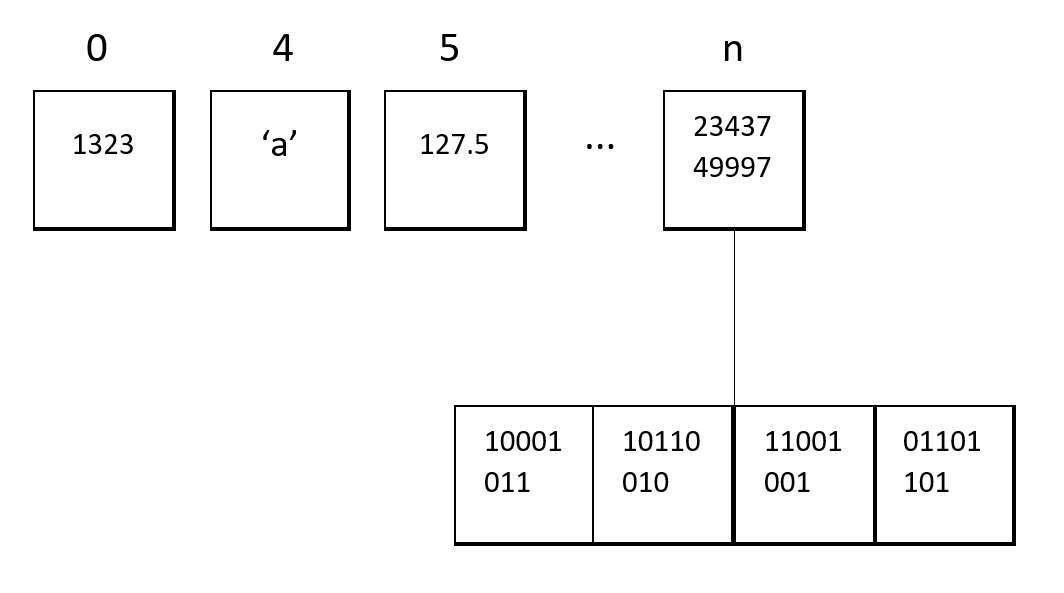
\includegraphics[scale=0.4]{Allocation.PNG}
		\caption{Memory Allocation of various data types}
		
	\end{figure}
	In Figure 1.1, the integer '1323' has taken 4 cubby holes or blocks sequentially from address '0' to '3'. Since a character is of 1 byte, character 'a' has taken only one cubby hole of address '4'.  The integer '234749997' has taken 4 cubby holes. Each cubby hole is of 8 bits or 1 byte. Therefore the binary representation of the integer is stored sequentially in the cubby holes. 
\newpage
\subsection{Conditional statements}
Conditional statements are used to make decisions based on a given condition.\\
\begin{figure}[H]
	\centering
	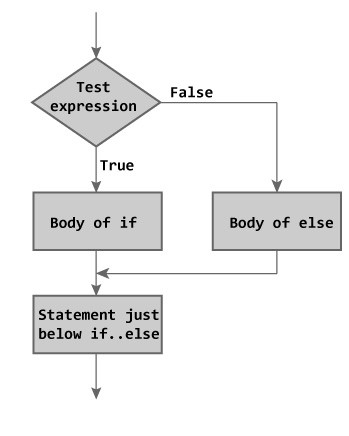
\includegraphics[scale=0.75]{if-else.jpg}
	\caption{Flowchart for if-else conditionals}
\end{figure}
~\\
\paragraph{Comparison operators with truth value}
Conditional statements works on the basis of the truth value of the expressions used.
There are multiple comparison operators which returns a truth value in boolean and are listed below. \\
\begin{table}[ht]
	\centering
	\begin{tabular}{|c|c|c|}
		\hline
		\thead{Operator} & \thead{Description} & \thead{Usage Example}\\
		\hline
		$==$ & equal to & \makecell{$1==1 \rightarrow$ true\\ 't' $==$ 'p' $\rightarrow$ false} \\
		\hline
		$!=$ & not equal to & \makecell{$5 != 5 \rightarrow$ false \\ $4.6 != 6.7 \rightarrow$ true }\\
		\hline
		$<$ & less than & \makecell{$5<4 \rightarrow$ false \\ 'a' $<$ 'b' $\rightarrow$ true ( using ASCII value)}\\
		\hline
		$<=$ & less than or equal to & \makecell{$4.5 <= 4.5 \rightarrow$ true \\ $3 <= 5.7 \rightarrow$ true }\\
		\hline
		$>=$& greater than or equal to & \makecell{'b' $>=$ 'b' $\rightarrow$ true \\ 
			true $>=$ false $\rightarrow$ true} \\
		\hline
		
	\end{tabular}
	\caption{Comparison operators}
	\label{tab:ComparisonOperators}
	
\end{table}
\begin{remark}
	Do not get confused between the assignment operator and equal to operator when using in an if conditional statement
\end{remark}
\newpage
The example below shows an example usage of if conditionals and comparison operators.
\begin{example}
	
	\begin{lstlisting}[title={Using if condition to check if number is divisible by 2},captionpos=b]
	#include <iostream>
	using namespace std;
	int main()
	{
	int num; //variable to store input
	cout<<"Enter number: "<<endl; //To show prompt
	cin>>num; //Taking and storing input value
	if(num % 2 == 0) //"a%b" to check the remainder when 'a' is  divided by 'b'
	{
	cout<<"Number is divisible by 2"<<endl;
	}
	else
	{
	cout<<"Number is not divisible by 2"<<endl;
	}
	return 0;
	}
	\end{lstlisting}
\end{example}
\subsection{Loops}
Loop is a sequence of instructions being repeated until a specific condition or target is reached. ~\\ ~\\
There are three types of loops in C++: \\
\paragraph{While loop}
A while loop statement repeatedly executes a target statement as long as a given condition is true. ~\\
The syntax of a while loop loop in C++ is:
\begin{lstlisting}
while (testExpression) 
{
	statement(s);
}
\end{lstlisting}
where, \textbf{testExpression} is checked on each entry of the while loop.
~\\ \\
Here is the flow of control in a while loop: \\
\begin{itemize}
\item The while loop evaluates the \textbf{test expression}.
If the \textbf{test expression} is true, codes inside the body of while loop is evaluated.
\item Then, the \textbf{test expression} is evaluated again. This process goes on until the \textbf{test expression} is false.
\item When the \textbf{test expression} is false, while loop is terminated.
\end{itemize}
\begin{figure}[H]
	\centering
	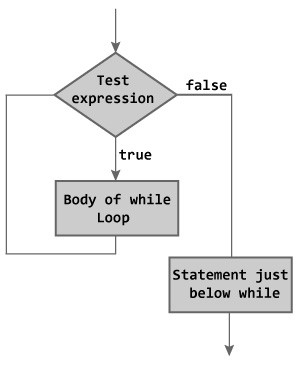
\includegraphics[scale=0.75]{while-loop.jpg}
	\caption{Flowchart of while loop}
\end{figure}
\begin{example}
	\begin{lstlisting}[title={Using While loop to increment an integer 5 times}, captionpos=b]
#include <iostream>
int main()
{
	int num = 1; //variable to be incremented
	int count = 0; //to keep track of number of iterations
	while(count < 5)
	{
		num = num + 1; //or num++ can also be used to increment
		count++;
	}
	return 0;
}
\end{lstlisting}
\end{example}
\paragraph{Do-while loop}
The syntax of do..while loop is:
\begin{lstlisting}
do {
	// codes;
}
while (testExpression);
\end{lstlisting}
Here is the flow of control in a while loop:
\begin{itemize}
\item The codes inside the body of loop is executed at least once. Then, only the \textbf{test expression} is checked.
\item If the \textbf{test expression} is true, the body of loop is executed. This process continues until the \textbf{test expression} becomes false.
\item When the \textbf{test expression} is false, do...while loop is terminated.
\end{itemize}
\begin{figure}[H]
	\centering
	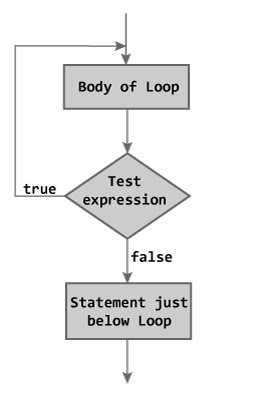
\includegraphics[scale=0.75]{dowhile-loop.jpg}
	\caption{Flowchart of do-while loop}
\end{figure}
\begin{example}
	\begin{lstlisting}[title={Using While loop to increment an integer 5 times}, captionpos=b]
#include <iostream>
int main()
{
	int num = 1; //variable to be incremented
	int count = 0; //to keep track of number of iterations
	do
	{
		num = num + 1; //or num++ can also be used to increment
		count++;
	}
	while(count<5)
	return 0;
}
\end{lstlisting}
\end{example}
\paragraph{For loop}
A for loop allows you to efficiently write a loop that needs to execute a specific number of times. ~\\
The syntax of a for loop in C++ is:
\begin{lstlisting}
for(initializationStatement; testExpression; updateStatement) 
{
	statement(s); 
}
\end{lstlisting}
Here is the flow of control in a for loop:
\begin{itemize}
\item The \textbf{initialization statement} is executed only once at the beginning.
\item Then, the \textbf{test expression} is evaluated.
If the \textbf{test expression} is false, for loop is terminated. But if the \textbf{test expression} is true, codes inside body of for loop is executed and \textbf{update statement} is executed.
\item Again, the \textbf{test expression} is evaluated and this process repeats until the \textbf{test expression} is false.
\end{itemize}
\begin{figure}[H]
	\centering
	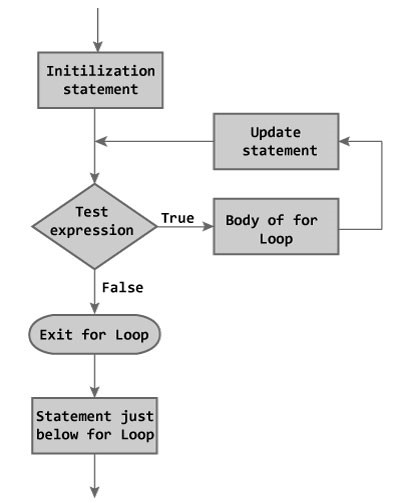
\includegraphics[scale=0.75]{for-loop.jpg}
	\caption{Flowchart of for loop}
\end{figure}
\begin{example}
	\begin{lstlisting}[title={Using For loop to increment an integer 5 times}, captionpos=b]
#include <iostream>
int main()
{
	int num = 1; //variable to be incremented
	for(int i = 0; i < 5; i++)
	{
		num = num + 1; //or num++ can also be used to increment
	}
	return 0;
}
\end{lstlisting}
\end{example}

\begin{example}
\begin{lstlisting}[title={Using While loop to increment an integer 5 times}, captionpos=b]
#include <iostream>
int main()
{
	int num = 1; //variable to be incremented
	int count = 0; //to keep track of number of iterations
	while(count < 5)
	{
		num = num + 1; //or num++ can also be used to increment
		count++;
	}
	return 0;
}
\end{lstlisting}
\end{example}
\newpage

\newpage
\subsection{Functions}
A function is a group of statements that together perform a task. Every C++ program has at least one function, which is main(), and all the most trivial programs can define additional functions.\\ ~\\ 
You can divide up your code into separate functions. How you divide up your code among different functions is up to you, but logically the division usually is such that each function performs a specific task. ~\\ ~\\
A function declaration tells the compiler about a function's name, return type, and parameters. A function definition provides the actual body of the function.
\paragraph{Defining a Function}
The general form of a C++ function definition is as follows:
\begin{lstlisting}
return_type function_name( parameter1, parameter2, parameter3,... ) 
{
	body of the function
}
\end{lstlisting} ~\\ ~\\
A C++ function definition consists of a function header and a function body. Here are all the parts of a function: ~\\
\begin{itemize}
\item \textbf{Return Type} - A function may return a value. The return\textunderscore type is the data type of the value the function returns. Some functions perform the desired operations without returning a value. In this case, the return\textunderscore type is the keyword void. \\
\item \textbf{Function Name} - This is the actual name of the function. The function name and the parameter list together constitute the function signature.\\
\item \textbf{Parameters} - A parameter is like a placeholder. When a function is invoked, you pass a value to the parameter. This value is referred to as actual parameter or argument. The parameter list refers to the type, order, and number of the parameters of a function. Parameters are optional; that is, a function may contain no parameters.\\
\item \textbf{Function Body} - The function body contains a collection of statements that define what the function does. ~\\
\end{itemize}

\paragraph{Declaring a function}
A function declaration tells the compiler about a function name and how to call the function. The actual body of the function can be defined separately.\\
\begin{lstlisting}
return_type function_name( parameter list );
\end{lstlisting}
\newpage
\paragraph{Calling a function}
While creating a C++ function, you give a definition of what the function has to do. To use a function, you will have to call or invoke that function. \\ ~\\
When a program calls a function, program control is transferred to the called function. A called function performs defined task and when it’s return statement is executed or when its function-ending closing brace is reached, it returns program control back to the main program. \\ ~\\
To call a function, you simply need to pass the required parameters along with function name, and if function returns a value, then you can store returned value.
\begin{example}
	\begin{lstlisting}[title={Declaration, definition amd calling of a max function},captionpos=b]
#include <iostream>
using namespace std;
	
// function declaration
int max(int num1, int num2);
	
int main () 
{
	// local variable declaration:
	int a = 100;
	int b = 200;
	int ret;
	
	// calling a function to get max value.
	ret = max(a, b);
	cout << "Max value is : " << ret << endl;
	
	return 0;
}
	
// function returning the max between two numbers
int max(int num1, int num2) 
{
	// local variable declaration
	int result;
	
	if (num1 > num2)
	result = num1;
	else
	result = num2;
	
	return result; 
}
	\end{lstlisting}
\end{example}
\newpage
\section{Problems}\index{Problems}
	\begin{problem}
		
		A certain grade of steel is graded according to the following conditions: ~\\
		\begin{itemize}
			\setlength\itemsep{1em}
			 \item Hardness must be greater than 50
			 \item Carbon content must be less than 0.7 \item Tensile strength must be greater than 5600
		\end{itemize}
		~\\ The grades are as follows: ~\\
		  \begin{itemize}
		  	\setlength\itemsep{1em}
		  \item Grade is 10 if all three conditions are met \item Grade is 9 if conditions (i) and (ii) are met
		  \item Grade is 8 if conditions (ii) and (iii) are met 
		  \item Grade is 7 if conditions (i) and (iii) are met
		  \item Grade is 6 if only one condition is met
		  \item Grade is 5 if none of the conditions are met
	\end{itemize}
		~\\Write a program, which will require the user to give values of hardness, carbon content and tensile strength of the steel under consideration and output the grade of the steel.
		\paragraph{Instructions}
		\begin{itemize}
			\item Use if-else conditional statements 
		\end{itemize}
	\end{problem}
~\\
\newpage
	\begin{problem}
		Two frogs named 'FrogPrime' and 'Frogatron' are in a well of depth 1000 feet. They decide to race each other to the top to see who is the winner.~\\ ~\\
		Both frogs can jump 4 feet at a time but slide down 1 foot every time, thus making the total distance covered to be 3 feet. ~\\ \\
		FrogPrime has a 2 \% chance to get an adrenaline rush and jump 5 feet.
		Frogatron has special claws that have a 2\% chance to grab on to a wall, thus it does not slide down 1 foot if the claws connect ~\\ \\
		The frogs will keep on jumping till one of them clears the well and is declared a winner. ~\\ \\
		Your program should simulate this behavior. It should find out the winner and report it. It should also report if there is a tie. ~\\ \\
		It should also display the progress of the frogs at every 50th jump.~\\ \\
		It should also display the total number of jumps once the competition is over. ~\\ \\
		The output should be similar to this:\\ \\
		\begin{center}
		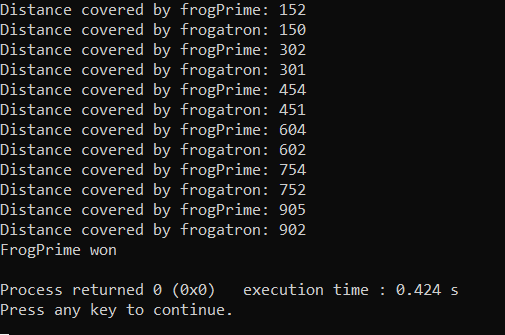
\includegraphics[scale=0.75]{Problem1_2.png}
		\end{center}
	\paragraph{Instructions}
	\begin{itemize}
		\item You can use random number generation to simulate chances. Find out yourself about using random number generation and ranges.
		\item Think in terms of loops and if-else conditionals
	\end{itemize}	
	
	\end{problem} ~\\ 
\begin{problem}
	Write a function IsPrime(int n) to test whether a parameter is prime. Apply the function in a program which prints all the prime numbers up to 100.
	\paragraph{Instructions}
	\begin{itemize}
		\item Use modulo operator to check divisibility
		\item You can use bool to keep check if a number is prime
		\item Break the question in parts and work on the function first
	\end{itemize}
\end{problem}
~\\
\begin{problem}
	Write a function Fibonacci(int n) which calculates the nth Fibonacci number. Write a main program that uses this function and the function from Problem 1.3 to print out the first 5 Fibonacci numbers that are also primes.
	\paragraph{Instructions}
	\begin{itemize}
		\item Think in terms of loops and an extensive use of variables to keep track of the needed terms in every iteration
	\end{itemize}
\end{problem}
\newpage
\section{Feedback}\index{Feedback}
\textbf{Please write the things you've learned from this lab and suggestions to make it more better and easy to learn.}



%----------------------------------------------------------------------------------------

\end{document}
